
\subsection{Utility classes}

\subsubsection{Exceptions}

\begin{figure}[!h]
  \centering
  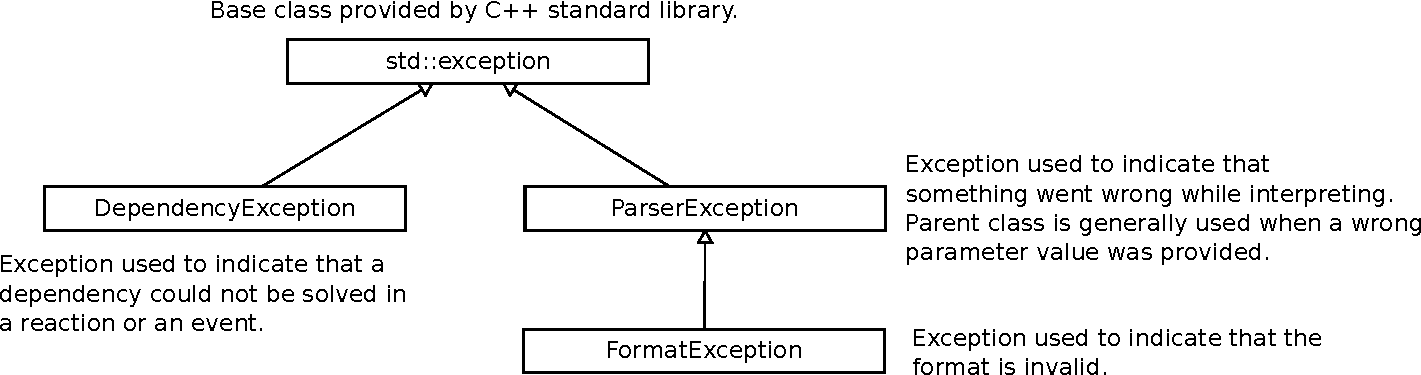
\includegraphics[width=\linewidth]{exception}
  \caption{Exceptions used in the simulator.}
  \label{fig:exception}
\end{figure}

Programming by contract (see Section~\ref{sec:tests}) covers most internal errors that might happen. Exceptions are only used when user input is treated. They are used to signify inconstencies in input files during the parsing step~\reffigp{fig:exception}.

\paragraph{Why are exceptions useful?} The nice thing about exceptions is that they can be caught and treated at a level that makes sense. In the parsing system, a format error is discovered by an \texttt{Interpreter}, which has no idea where the input line comes from and could not display a useful error message on its own. It is caught at the \texttt{Parser} level, enriched with information about input file, input line and so on, before being displayed.

\paragraph{Perspectives} Errors occurring during simulation are displayed without using exceptions and suffer the bias described above. If a \texttt{Release} fails, there is a low level message such as ``Unknown product''. We could throw an exception and catch it at the \texttt{Simulation} level, then use \texttt{CellState} to get the name of the \texttt{ChemicalSequence}, the \texttt{ProductTable} and the polymerase involved in the \texttt{Release}, providing useful information for the user.

\subsubsection{Random handler}

\begin{figure}[!h]
  \centering
  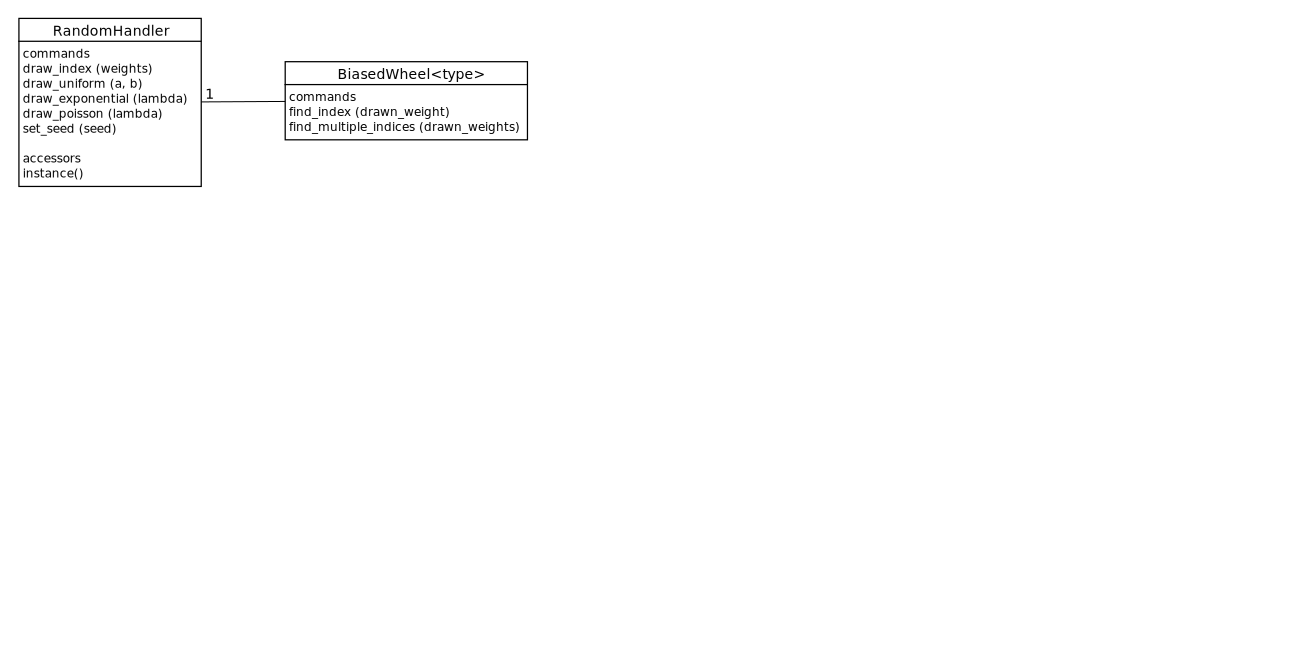
\includegraphics[width=0.8\linewidth]{randomhandler}
  \caption{\texttt{RandomHandler} and \texttt{BiasedWheel} used for multinomial drawing. \texttt{RandomHandler} uses the Singleton pattern, meaning exactly one instance of the class is created and used throughout the simulator. It has to be accessed using \texttt{RandomHandler::instance()}.}
  \label{fig:random_handler}
\end{figure}

A unique \texttt{RandomHandler} is used throughout the simulation to control the random seed by using a Singleton pattern~\reffigp{fig:random_handler}.

\subsubsection{Factories}

\begin{figure}[!h]
  \centering
  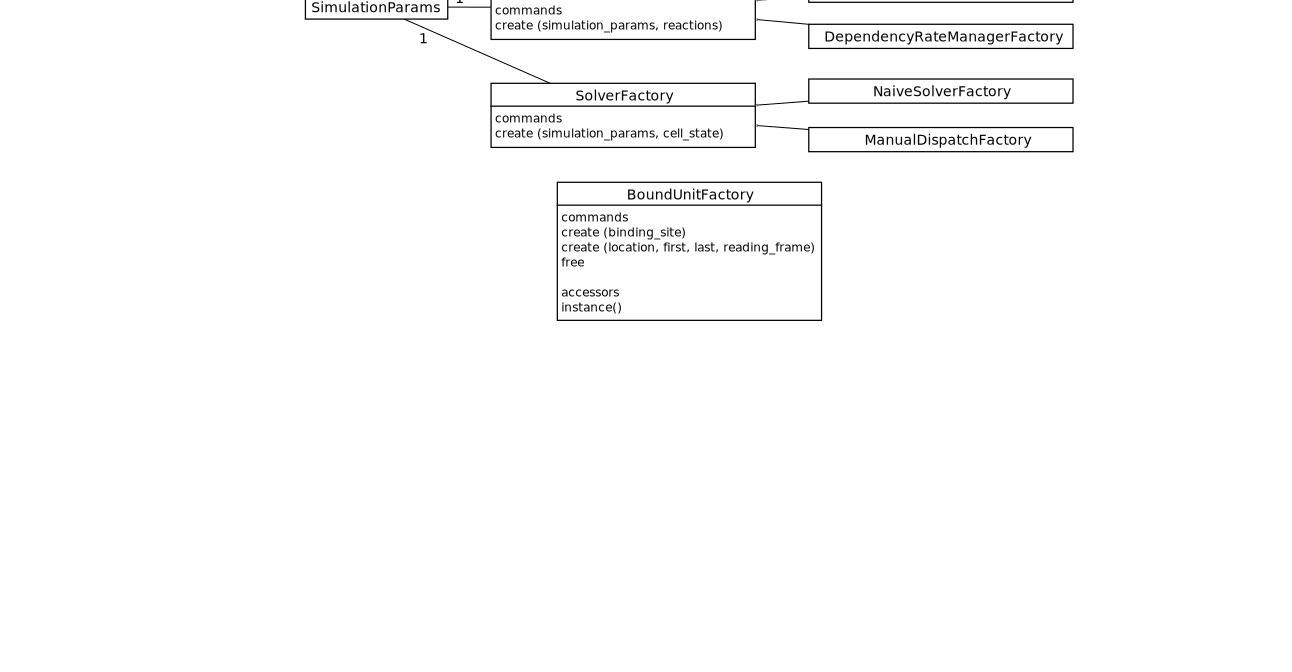
\includegraphics[width=\linewidth]{factories}
  \caption{\texttt{RateContainerFactory}, \texttt{RateManagerFactory} and \texttt{SolverFactory} are used by \texttt{SimulationParams} to record what \texttt{RateContainer}, \texttt{RateManager} and \texttt{Solver} the user wishes to use (Abstract Factory Pattern). \texttt{BoundUnitFactory} is used to control memory usage by \texttt{BoundUnit}s.It enables recycling of bound units, avoiding memory reallocation. It uses the Singleton pattern to make sure all instances of \texttt{BoundUnit}s are stored at the same place.}
  \label{fig:factories}
\end{figure}

Factories are used to remember user options and handle memory more efficiently~\reffigp{fig:factories}.

\paragraph{Why are factories useful?} First, we have a context problem. For example, \texttt{SimulationParams} knows what kind of \texttt{RateContainer} the user wishes to use, but cannot instantiate it because it lacks parameters to instantiate it (the number of reactions in the system) and would not know where to instantiate it. The naive way of doing would be recording a string saying for example \texttt{``HybridRateContainer''} then use a \texttt{if} structure at the right place to instantiate the correct \texttt{RateContainer}. \emph{This is bad!} This means that every time a new \texttt{RateContainer} is added/removed, we have to track down every place in the program where a \texttt{RateContainer} is used and modify the \texttt{if} structure. In object-oriented programming we want to avoid the use of such structures because of such maintenance problem. This is done by using inheritance and factories. There is a \texttt{if} structure in \texttt{SimulationParams} to create the correct factory, this factory is passed as an abstract \texttt{RateContainerFactory} to client classes. Clients have no idea how many variants of the factory there are and they should not care, they just call \texttt{create()} on it, no \texttt{if}s involved. When a new \texttt{RateContainer} is added, we add a new child to \texttt{RateContainerFactory} and adapt the \texttt{if} structure in \texttt{SimulationParams}, \emph{but literally nothing changes in the code of client class}. Factories = better maintenance (Abstract Factory pattern).

\subsubsection{Vector-based containers}

The simulator uses two non-standard containers, \texttt{VectorList} and \texttt{VectorQueue}. A typical example is a \texttt{BoundChemical} storing all its \texttt{BoundUnit}s. There is typically a high turnover of bound units and units reacting are drawn uniformly within the list of bound units. Naively, we would use a list to perform such a task, but there are huge performance issues. Using standard C++ \texttt{std::list} would imply a lot of memory reallocation each time a \texttt{BoundUnit} is added/removed (because a node of the list is created/deleted). What is more, if, by random drawing, we decide that it is the 10th unit that is going to react, we need to loop through 10 elements before accessing the correct element.

Using a \texttt{std::list} has a \emph{huge} impact on performance. Therefore, in \texttt{BoundChemical} (and a lot of other places in the program), we replace \texttt{std::list} by a \texttt{VectorList}, where elements are placed in a \texttt{std::vector}. There is one trick to use: every time an element is removed, it is replaced by the last element in the vector, so that elements remain contiguous in memory. This means that order of elements is lost, but in the example above and every time we \texttt{VectorList}, order is not important. The size of \texttt{std::vector} is automatically adjusted by C++. Most of the time it will be larger than the number of elements it contains, but we prefer using a little more memory than contantly reallocating nodes. What is more, accessing the nth element is instantaneous.

The same general idea applies for \texttt{VectorQueue} except we need to know in advance how large the queue will be. It is used to update nodes in \texttt{RateTree} because we know how many nodes there are in the tree and they are updated at most once.

\subsubsection{Handler classes for memory handling}

C++ has no garbage collector and this program was designed according to old standards (that is without smart pointers). Therefore, we need to be extremely careful to delete elements at the right time. This is achieved by using as few storage places as possible. As described earlier, \texttt{CellState} is used to store all reactions and reactants read from files. We designed a \texttt{Handler} class that effectively stores objects to their definitive location and distributes references or pointers to this constant location. Similarly \texttt{EventHandler} and \texttt{BoundUnitFactory} are used to store \texttt{Event}s and \texttt{BoundUnit}s which are the other dynamical elements stored in the program. At the end of the simulation, all these handlers have to be carefully deleted. Observer patterns are particularly dangerous, as we must be sure that at destruction, there is no message sent to a non-existent observer. Every time an observer pattern is used, we made sure that observers are correctly unsuscribed when they are destructed or the object they observe is destructed.
